\documentclass{csri19}

%%% Starting page will be changed when we combine the proceedings
\setcounter{page}{3}

% PACKAGES ---------------------------------------------------------------
\usepackage{amsfonts,amsmath,graphicx,subfigure}
% ADD YOUR OWN PACKAGES HERE ---------------------------------------------
\usepackage{mathtools, amssymb}

% DEFINITIONS ------------------------------------------------------------
% ADD YOUR OWN DEFINITIONS HERE ------------------------------------------
% BE SURE TO PREFACE LABEL WITH YOUR OWN INITIALS (SSS in this example) --
\newcommand{\SSSnorm}[1]{\left\Vert#1\right\Vert}
\newcommand{\SSSabs}[1]{\left\vert#1\right\vert}
\newcommand{\CFKg}{\mathfrak{g}}

% This controls the table-of-contents entry in the proceedings. Edit it
% to include your article title followed by the authors' names, as shown.
\addcontentsline{toc}{chapter}{Exponential Integrators for the Energy 
Exascale Earth System Model\\
{\em C.F.\ Krause and A.J.\ Steyer}}

\pagestyle{myheadings}

\thispagestyle{plain}

% This gives the running head. Usually you list a shortened version of
% your article title (unless it's already very short) along with
% the author's names, as shown.
\markboth{Exponential Integrators for E3SM}{C.F.\ Krause and A.J.\ Steyer}

% Put your article title in here
\title{Exponential Integrators for the Energy Exascale Earth System Model}

% List each author, their affiliation, and their e-mail address, as shown.
\author{Cassidy F.\ Krause\thanks{University of Kansas, ckrause@ku.edu}
\and Andrew J.\ Steyer\thanks{Sandia National Laboratories, asteyer@sandia.gov}}

\begin{document}
\maketitle

% Include your abstract here.
\begin{abstract}
The HOMME-NH nonhydrostatic atmosphere model has a system of stiff ODEs 
which are currently solved using implicit-explicit (IMEX) Runge-Kutta (RK) 
methods. We introduce a horizontally explicit - vertically integrating 
factor exponential method (HEVI-Exponential) as an alternative to solving 
these stiff equations. The main drawback to exponential methods is the cost
of forming the matrix exponential. Here, we show that we can mitigate this 
cost by taking advantage of the tridiagonal-like form of our Jacobian and 
parallelizing our computations, making this solver an attractive option for
HOMME-NH.
\end{abstract}

\section{Introduction} \label{CFK:sec:intro}
Stiff ODEs are notorious for requiring a very small step size when solved 
explicitly. Because this restriction can make algorithms quite inefficient,
 two different methods have been developed for dealing with these problems. 

Suppose we have an ODE given by \[ f(u) = s(u) + n(u),\] where $s(u)$ 
contains the stiff part of the equation, and $n(u)$ contains the nonstiff 
part. One way to deal with this problem is to use an implicit Runge-Kutta
method on the stiff part, and an explicit Runge-Kutta on the nonstiff part. 
This is the current method used in the HOMME-NH nonhydrostatic atmosphere 
model of the E3SM, and it performs quite well.

Another approach is to use an exponential-type integrator, such as 
integrating factor Runge-Kutta methods (IFRKs). In this case, we split our
 method as \[ f(u) = Lu + N(u),\] where $L$ is a linear operator containing
 the stiff part of the ODE, and $N(u) = f(u) - Lu$ contains the nonstiff 
terms. Often, $L = f'(u)$, but we do not assume this is the case. 

Using the change of variables $v(t) = e^{-L(t-t_m)}u(t)$, we have
\begin{equation}\label{CFK:eqn:vode}
v_t = e^{-L(t-t_m)}N(e^{L(t-t_m)}v).
\end{equation} 
We can then apply an $r-$stage Runge-Kutta method to solve 
\ref{CFK:eqn:vode}, as discussed in section \ref{CFK:sec:implementation}. 
In this paper, we implement these exponential-type methods in the HOMME-NH
 model as a feasible alternative to the IMEX Runge-Kutta methods.

The rest of the paper is structured as follows: In section 
\ref{CFK:sec:homme}, we give a brief background of the non-hydrostatic 
model; section \ref{CFK:sec:matexp} discusses exponential integrator 
methods; the implementation of these methods is given in section 
\ref{CFK:sec:implementation}; and numerical results are given in section 
\ref{CFK:sec:results}.

\section{HOMME-NH}\label{CFK:sec:homme}
In the HOMME-NH model, we employ a horizontally explicit, vertically 
implicit (HEVI) partitioning. Choosing to linearize around the stiffly 
treated terms, we can write the governing equations as
\[q_t \coloneqq \begin{bmatrix} u_t \\
w_t\\
\phi_t\\
\theta_t\\
\frac{\partial \pi}{\partial \eta}
\end{bmatrix} = n(q) + s(q) \equiv n(q) + \begin{bmatrix}
0\\
-\CFKg (1-\mu)\\
\CFKg w\\
0\\
0\end{bmatrix},\] 
where $w, u,\phi, \theta,$ and $\frac{\partial \pi}{\partial \eta}$ are the
 state variables in the HOMME-NH model, as listed in table \ref{CFK:tab:variables}.

\begin{table}
  \caption{Variables in HOMME-NH}
  \label{CFK:tab:variables}
  \begin{center}
    \begin{tabular}{|c|l|}
      \hline
      \textbf{Variable Name} & \textbf{Description} \\
      \hline
      $w$ & Vertical velocity \\
      $u$ & \\
      $\phi$ & Geopotential \\
      $\theta$ & Potential temperature \\
      $\frac{\partial\pi}{\partial\eta}$ & \\
      \hline 
    \end{tabular}
  \end{center}
\end{table}

Linearizing $s(q)$ gives the following Jacobian:
\[ J = \begin{bmatrix}
 &                  &                                                   &  & \\
 & 0                & \CFKg \Delta t \frac{\partial \mu}{\partial \phi} &  & \\
 & \CFKg \Delta t I & 0                                                 &  & \\
 &                  &                                                   &  & \\
 &                  &                                                   &  & \end{bmatrix}.\]

So, forming $e^{\alpha J}$ reduces to forming an exponential of 
\[ \begin{bmatrix}
   0              & \CFKg \Delta t \frac{\partial \mu}{\partial \phi} \\
 \CFKg \Delta t I & 0  \end{bmatrix},\]
where $\dfrac{\partial \mu}{\partial \phi}$ is tridiagonal. The most 
computationally expensive part of exponential-type methods is forming the 
matrix exponential; as discussed in the next section, we are able to 
leverage the structure of this particular Jacobian in order to develop 
methods that are competitive with the currently implemented IMEX Runge-
Kutta methods.

\subsection{The Matrix Exponential}\label{CFK:sec:matexp} 
One can form the matrix exponential analytically if the matrix $A$ is 
diagonalizable, but finding the eigenvalues of $A$ is expensive, and it is
 not generally guaranteed that $A$ is diagonalizable. A more general 
approach is to approximate $e^{A}$ using a Pad\'e or Taylor series 
approximation. Other methods of approximating the matrix exponential are 
discussed in \cite{CFK:Moler2003}.

We choose to implement a $(p,q)$-Pad\'e approximation 
$e^{A}\approx \left[Q_{pq}(A)\right]^{-1}P_{pq}(A)$, where $P_{pq}(A)$ and 
$Q_{pq}(A)$ are defined as follows:

\begin{align*}
P_{pq}(A) &= \sum_{j=1}^p\frac{(p+q-j)!p!}{(p+q)!j!(p-j)!}A^j\\
Q_{pq}(A) &= \sum_{j=1}^q\frac{(p+q-j)!q!}{(p+q)!j!(q-j)!}(-A)^j
\end{align*}

The error for this approximation is given by
\[ e^A - \left[Q_{pq}(A)\right]^{-1}P_{pq}(A) = \mathcal{O}(A^{p+q+1}).\]

If the matrix $A$ has eigenvalues that are spread far apart, this 
approximation can be rather inaccuarate. To mitigate this problem, we 
implement a scaling and squaring approach. Because of the properties of 
matrix exponentials, we can write
\[e^{A} = \left(e^{A/k}\right)^k,\]
where $k$ is chosen to be the smallest power of $2$ so that 
$\|A/k\| \leq 0.5$. With this factorization, the matrix $A$ is scaled down
 to $A/k$, and the matrix exponential $e^{A/k}$ is calculated using the 
formulas above. This matrix exponential is then squared repeatedly to 
recover the desired matrix exponential $e^{A}$.

Once the terms $P_{pq}$ and $Q_{pq}$ are calculated, the product 
$\left[Q_{pq}(A)\right]^{-1}P_{pq}(A)$ is a potentially expensive 
computation. Fortunately, for our problem, the matrix $A$ we consider has a
 special structure. It is of the form 
\[A= \begin{bmatrix} 0 & \alpha T\\
  \alpha I & 0 \end{bmatrix},\]
where $T$ is tridiagonal. This form allows us to solve 
$\left[Q_{pq}(A)\right]^{-1}P_{pq}(A)$ using tridiagonal solves and back 
substitution.

To do so, we first factor $Q_{pq}(A)$ as
\[ Q_{pq}(A) = \prod_{j=1}^q\left[\sigma_jI-A\right]\text{, where }\sigma_j\in \mathbb{C}\text{ for }j=1,\dots,q.\]

Then, since we want to solve for 
$R \coloneqq \left[Q_{pq}(A)\right]^{-1}P_{pq}(A)$, we have
\begin{align*}
Q_{pq}(A) R &= P_{pq}(A)\\
\prod_{j=1}^q\left[\sigma_jI-A\right]R &= P_{pq}(A).
\end{align*}

Define $R_1 \coloneqq \left[\sigma_2I-A\right]\left[\sigma_3I-A\right]\cdots\left[\sigma_qI-A\right]R$.
Then our equation becomes
\[ \left[\sigma_1I-A\right]R_1 = P_{pq}(A).\] Since $\left[\sigma_1I-A\right]$ 
is a tridiagonal matrix, we can solve for $R_1$ using far fewer operations
 than if $\left[\sigma_1I-A\right]$ were a full matrix.

Now we have
\[\left[\sigma_2I-A\right]\left[\sigma_3I-A\right]\cdots\left[\sigma_qI-A\right]R = R_1.\] 
We can continue in this way, defining 
$R_j \coloneqq \left[\sigma_{j+1}I-A\right]\left[\sigma_{j+2}I-A\right]\cdots\left[\sigma_qI-A\right]R$
 and solving
\[\left[\sigma_jI-A\right]R_j = R_{j-1}\] 
for $R_j$, until we arive at
\[\left[\sigma_qI-A\right]R = R_{q-1}.\] 
Solving this last tridiagonal system gives us the $R = \left[Q_{pq}(A)\right]^{-1}P_{pq}(A)$
 that we are looking for.

This approach is particularly efficient if the values of $p$ and $q$ are 
small, so that we can analytically find $\{\sigma_j\}_{j=1}^q$ ahead of 
time. Of course, approximations like this do rather poorly for ill-
conditioned matrices, so we must validate that these approximations work 
for the Jacobians we are interested in. To validate the Pad\'e 
approximation, we let the model spin up and consider the Jacobian at that
time. For this model, our Jacobian will have unique, purely imaginary
eigenvalues, so we can calculate the matrix exponential analytically, and 
compare it to our approximation. The following table gives the results of
 several diagonal $(p,q)$-Pad\'e approximations, for different values of
$p=q$.
\begin{table}[ht]
  \begin{center}
    \caption{Error of Pad\'e Approximation}
    \label{CFK:tab:PadeError}
    \begin{tabular}{|c|c|}
      \hline
      \textbf{Value of $p=q$} & \textbf{Error}\\
      \hline
      2 & 1.30e-10 \\
      3 & 5.25e-13 \\
      4 & 4.92e-13 \\
      5 & 5.42e-13 \\
      \hline
    \end{tabular}
  \end{center}
\end{table}

Since a $(2,2)$-Pad\'e approximation yields a considerably accurate matrix 
exponential and also gives the benefit of taking advantage of the 
tridiagonal structure, we choose to implement this method.

The implementation of HOMME-NH means that $\frac{\partial\mu}{\partial\phi}$
 is tridiagonal.  Forming the exponential via Pad\'e approximation then 
requires inverting a matrix of the following form:
\[\begin{bmatrix} 0 & \CFKg\Delta t\frac{\partial\mu}{\partial\phi} \\
    \CFKg\Delta t I & 0 \end{bmatrix} =
 \begin{bmatrix} \sigma I  & -\CFKg\Delta t \frac{\partial\mu}{\partial\phi} \\
 -\CFKg\Delta t I          & \sigma I \end{bmatrix}.\]
Consider the following linear equation:
\[\begin{bmatrix} \sigma I  & -\CFKg\Delta t \frac{\partial\mu}{\partial\phi} \\
           -\CFKg\Delta t I & \sigma I \end{bmatrix}
\begin{bmatrix} Z_1 \\
 Z_2 \end{bmatrix} = 
\begin{bmatrix} P_1 \\
 P_2 \end{bmatrix}.\]
If $\sigma = 0$ this decomposes to a tridiagonal linear solve and a trivial solve. 
If $\sigma \neq 0$, then we left multiply by $\begin{bmatrix} I & 0 \\
                                     \CFKg\Delta t \sigma^{-1}I & I \end{bmatrix}$ to obtain:
\[\begin{bmatrix} 
 \sigma I  & -\CFKg\Delta t \frac{\partial\mu}{\partial\phi} \\
         0 & \sigma I -\left(\CFKg\Delta t\right)^2  \sigma^{-1}\frac{\partial\mu}{\partial\phi}
 \end{bmatrix}
 \begin{bmatrix} Z_1 \\
 Z_2 \end{bmatrix} = 
\begin{bmatrix} P_1 \\
 \CFKg\Delta t \sigma^{-1} P_1 +  P_2 \end{bmatrix}.\]
The matrix $\sigma I -\left(\CFKg\Delta t\right)^2\sigma^{-1}\frac{\partial\mu}{\partial\phi}$ 
is tridiagonal since $\frac{\partial\mu}{\partial\phi}$ is tridiagonal. 
Therefore we can solve for $X_2$ with a tridiagonal solve of 
\[\left[\sigma I -\left(\CFKg\Delta t \right)^2  \sigma^{-1}\frac{\partial\mu}{\partial\phi}\right]Z_2
 = \CFKg\Delta t\sigma^{-1} P_1 +  P_2\]
and then form $Z_1$ as 
\[Z_1 = \sigma^{-1}\left[P_1 + \CFKg\Delta t\frac{\partial \mu}{\partial \phi}\right] Z_2.\]

\section{Implementation}\label{CFK:sec:implementation}
We consider several explicit Runge-Kutta methods to solve equation 
\ref{CFK:eqn:vode}. We consider several Runge-Kutta methods given by the 
following Butcher tableaux:
\[
 \begin{array}{c|ccc}
0   & 0   & 0 & 0\\
1/2 & 1/2 & 0 & 0\\
1   & 0   & 1 & 0\\
\hline
    & 0   & 1 & 0
\end{array}\qquad
\begin{array}{c|cccc}
0   & 0   & 0   & 0 & 0\\
1/2 & 1/2 & 0   & 0 & 0\\
1/2 & 0   & 1/2 & 0 & 0\\
1   & 0   & 0   & 1 & 0\\
\hline
    & 0   & 0   & 1 & 0
\end{array}\qquad
\begin{array}{c|cccccc}
0   & 0   & 0   & 0   & 0   & 0   & 0\\
1/5 & 1/5 & 0   & 0   & 0   & 0   & 0\\
1/5 & 0   & 1/5 & 0   & 0   & 0   & 0\\
1/3 & 0   & 0   & 1/3 & 0   & 0   & 0\\
2/3 & 0   & 0   & 0   & 2/3 & 0   & 0\\
1   & 1/4 & 0   & 0   & 0   & 3/4 & 0\\
\hline
    & 1/4 & 0   & 0   & 0   & 3/4 & 0
\end{array}
\]

\section{Results}\label{CFK:sec:results}
Convergence test:
\begin{figure}[hbh]
\label{CFK:fig:convtest}
\begin{center}
\begin{tabular}{cc}
\scalebox{0.2}{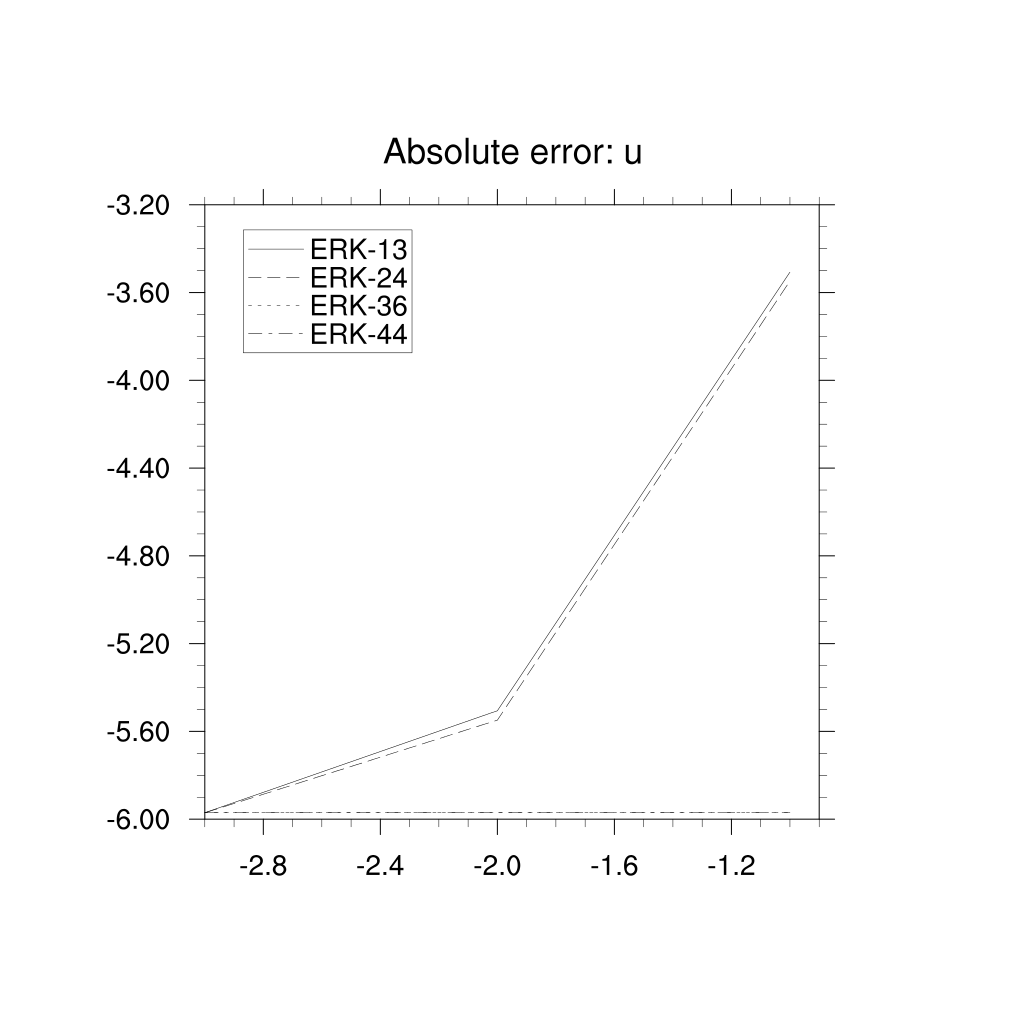
\includegraphics{plots/CFKu_err.png}} 
&
\scalebox{0.2}{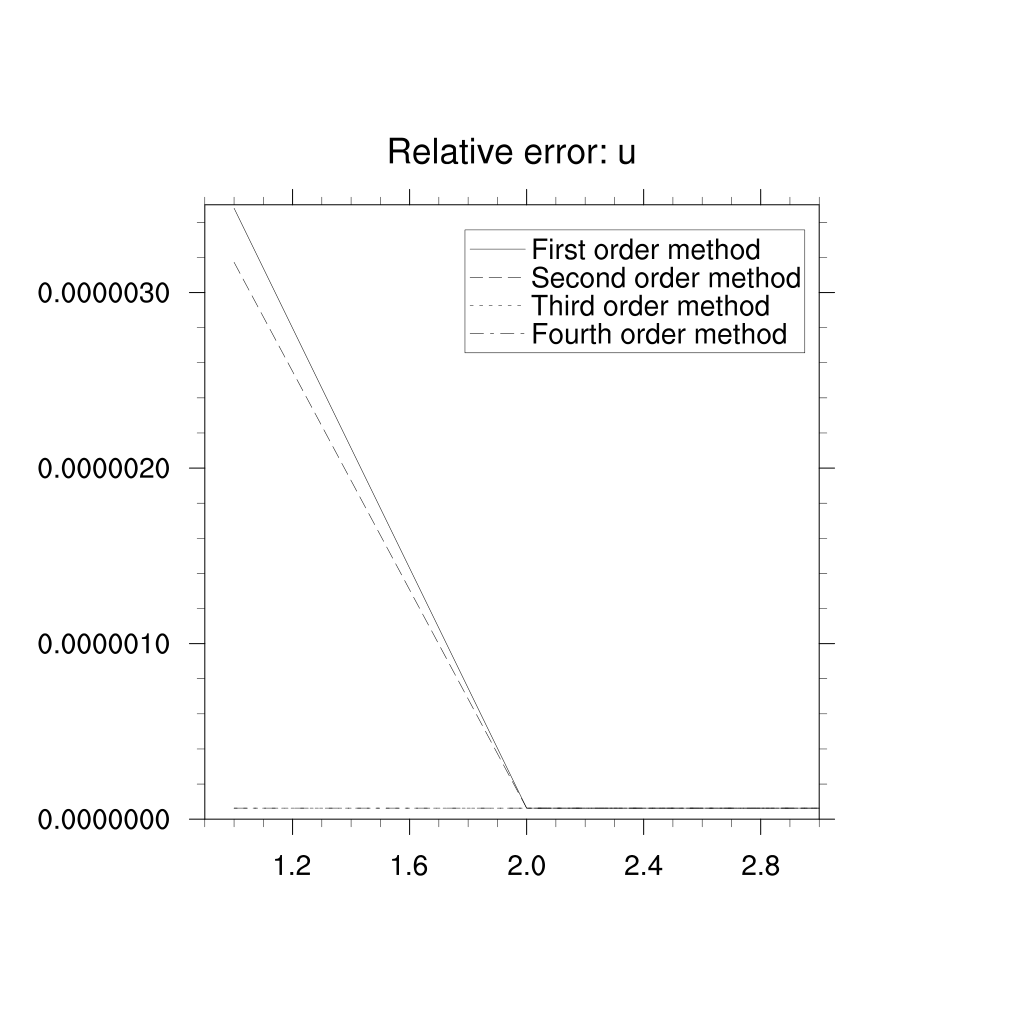
\includegraphics{plots/CFKu_err_rel.png}}
\\
\scalebox{0.2}{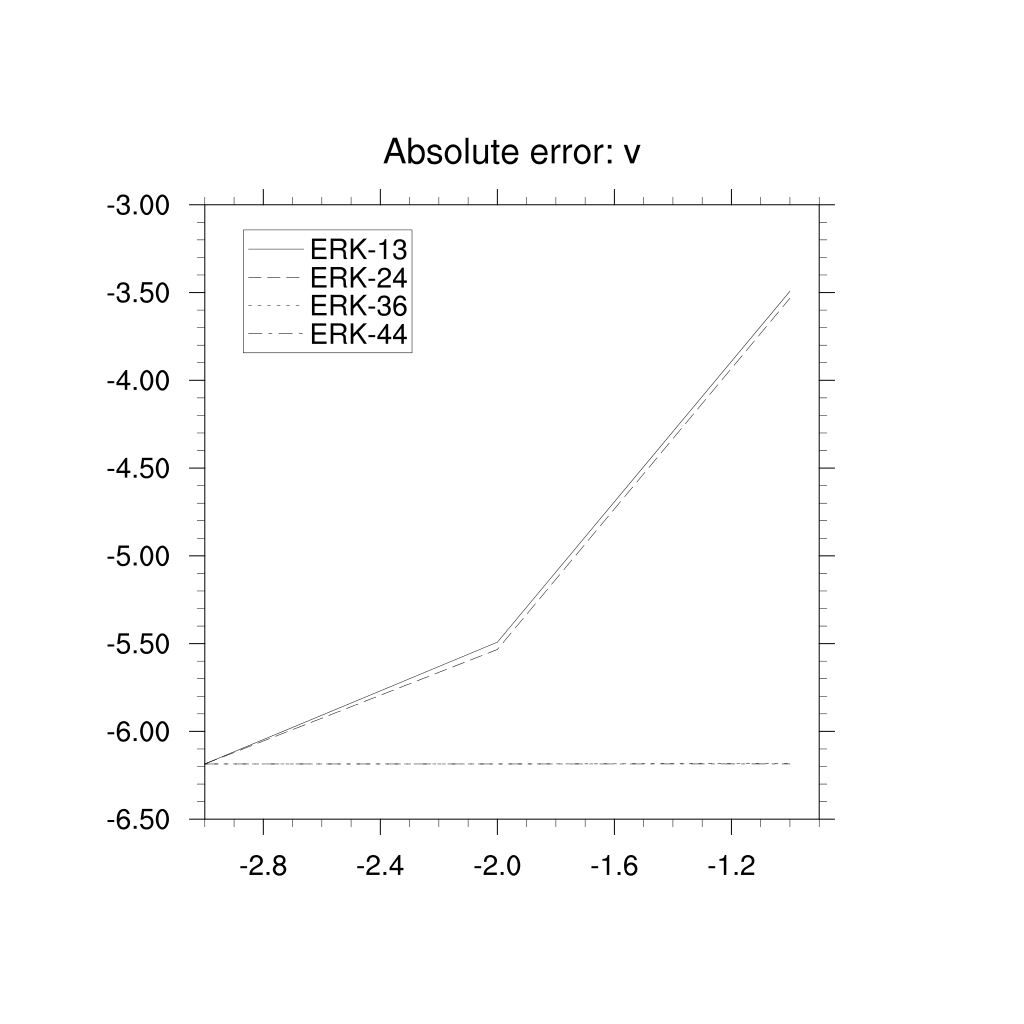
\includegraphics{plots/CFKv_err.png}} 
&
\scalebox{0.2}{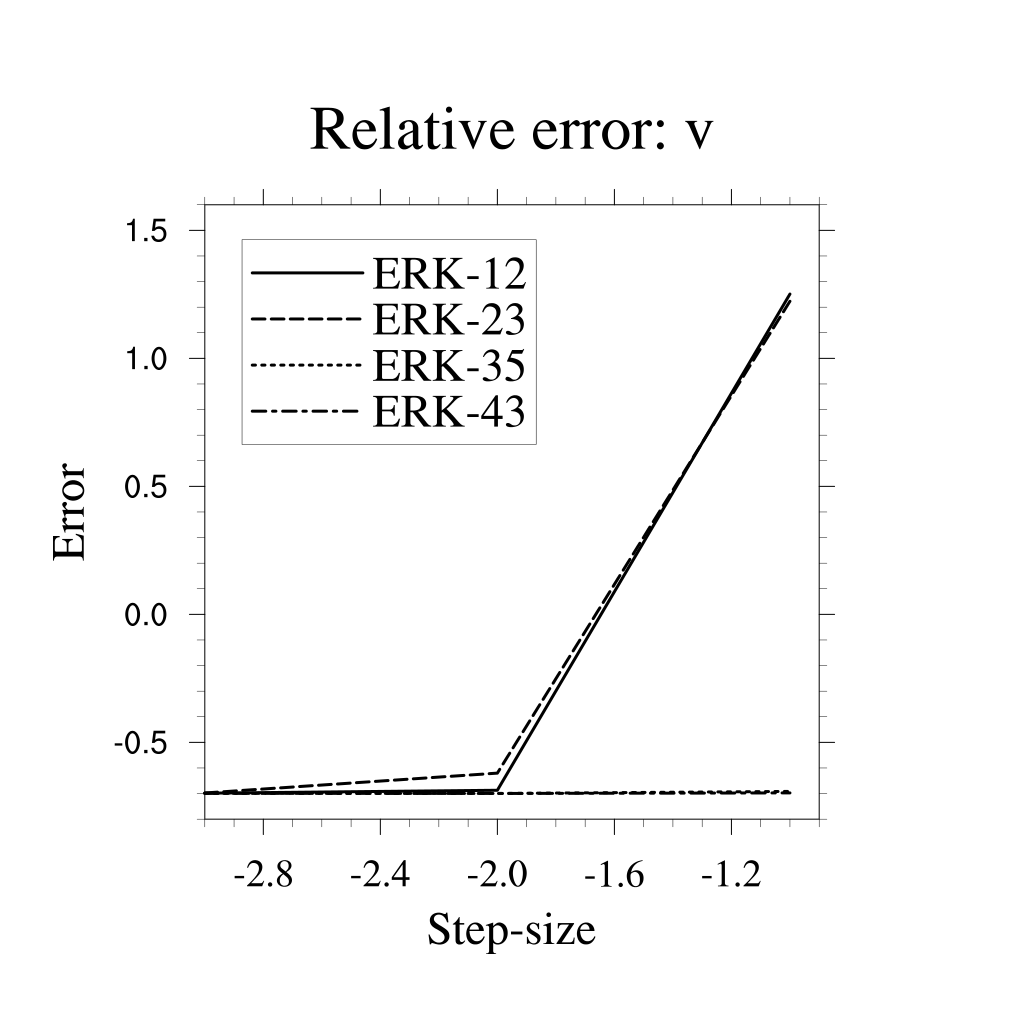
\includegraphics{plots/CFKv_err_rel.png}}
\end{tabular}
\end{center}
\caption{Errors with exponential integrating factor methods.}
\end{figure}

\begin{figure}[hbh]
\label{CFK:fig:convtest1}
\begin{center}
\begin{tabular}{cc}
\scalebox{0.2}{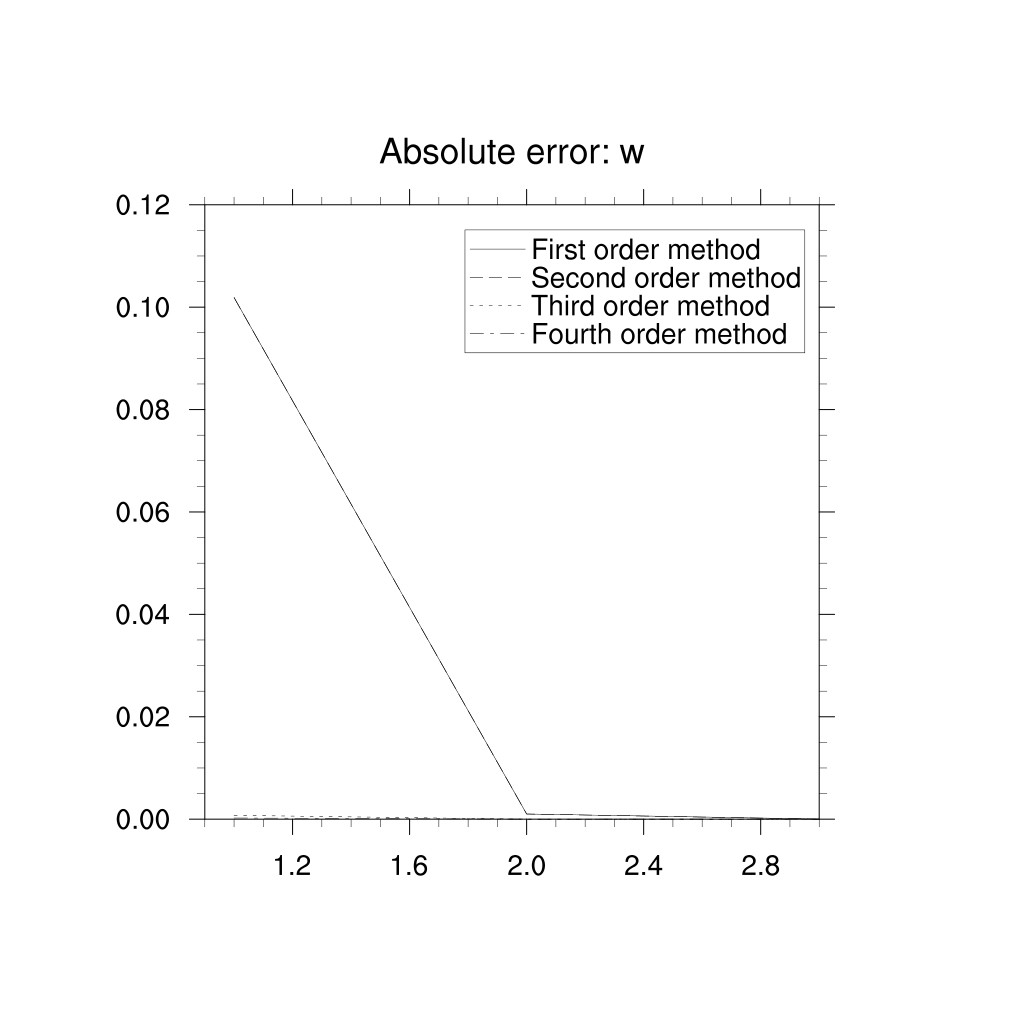
\includegraphics{plots/CFKw_err.png}} 
&
\scalebox{0.2}{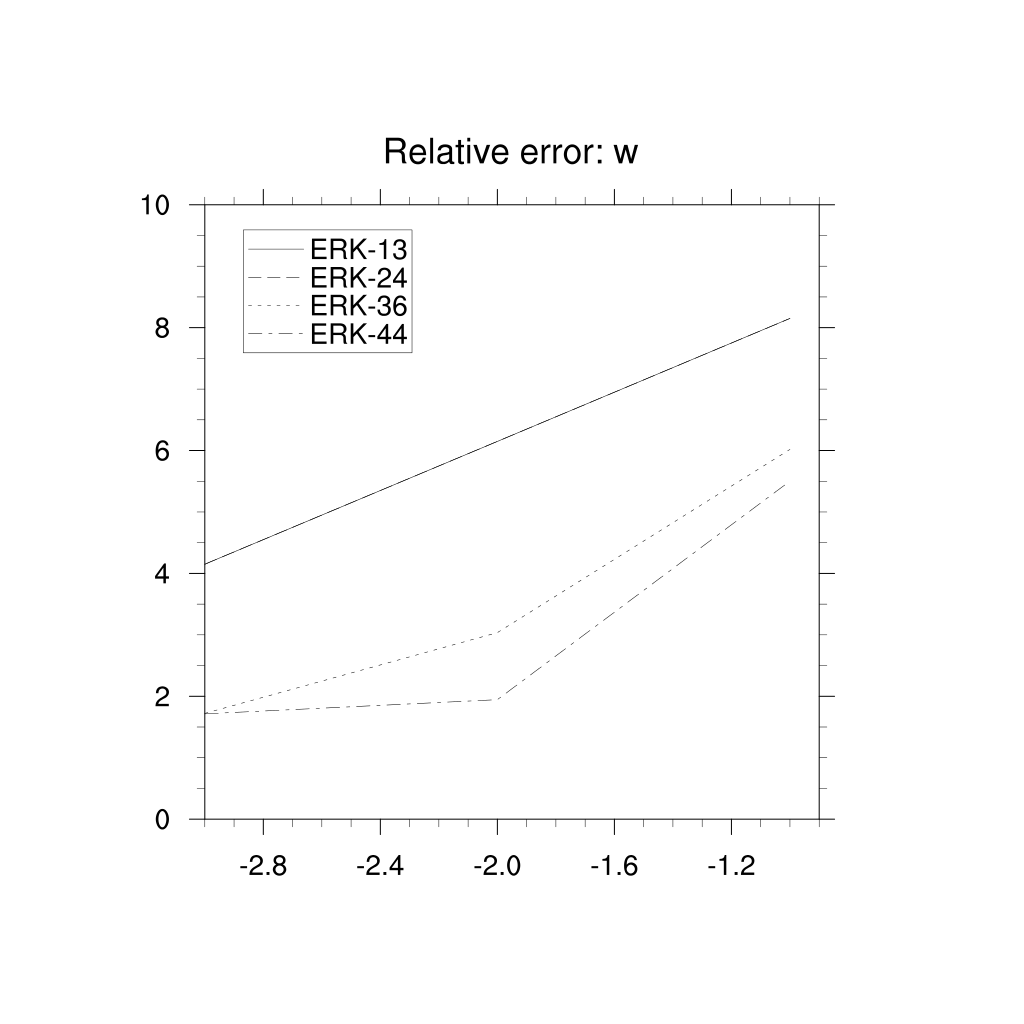
\includegraphics{plots/CFKw_err_rel.png}}
\\
\scalebox{0.2}{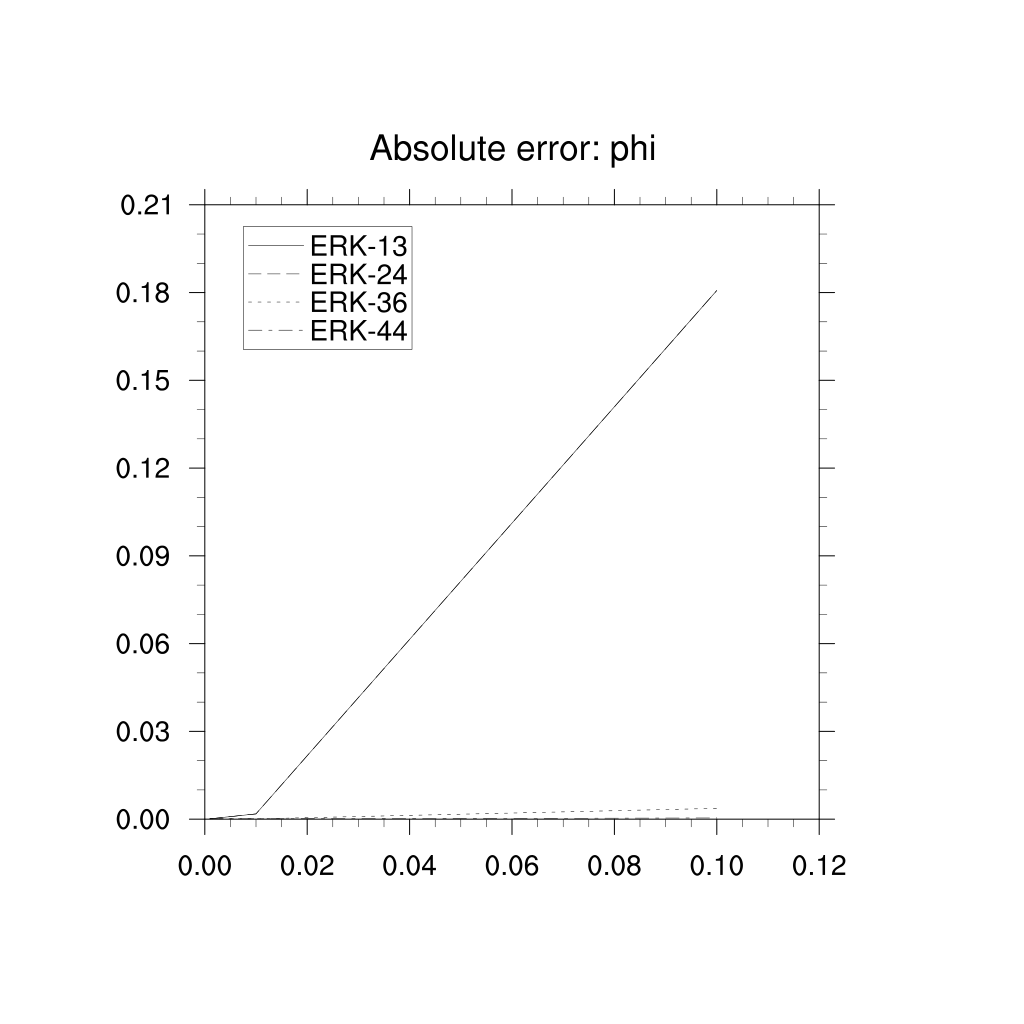
\includegraphics{plots/CFKphi_err.png}} 
&
\scalebox{0.2}{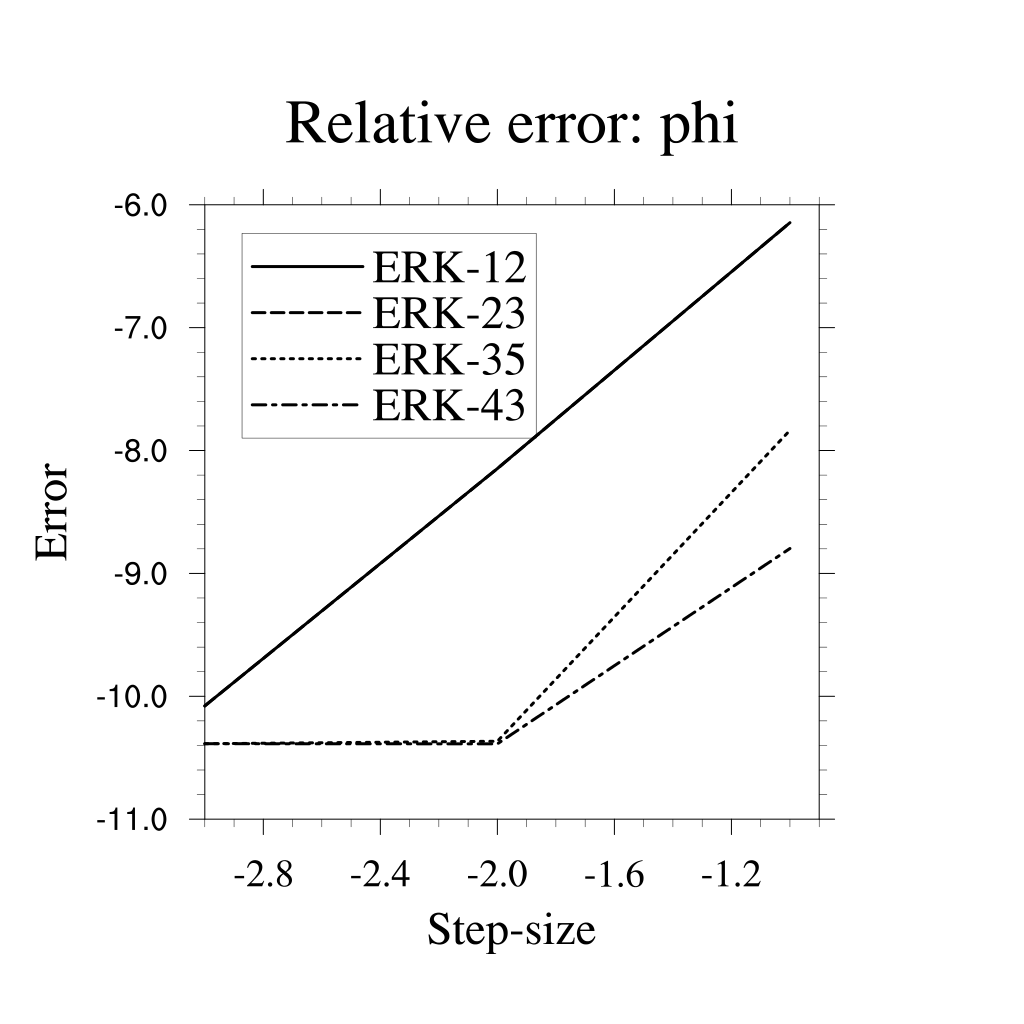
\includegraphics{plots/CFKphi_err_rel.png}}
\end{tabular}
\end{center}
\caption{Errors with exponential integrating factor methods.}
\end{figure}

\section{Conclusions}

\bibliographystyle{siam}
% Edit the line below to be your first and last names.
\bibliography{CassidyKrause}

% Edit FirstnameLastname below to be your first and last names, but leave the line commented out.
% This line will help me merge bibliographies for the proceedings.
%\documentclass{csri19}

%%% Starting page will be changed when we combine the proceedings
\setcounter{page}{3}

% PACKAGES ---------------------------------------------------------------
\usepackage{amsfonts,amsmath,graphicx,subfigure}
% ADD YOUR OWN PACKAGES HERE ---------------------------------------------
\usepackage{mathtools, amssymb}

% DEFINITIONS ------------------------------------------------------------
% ADD YOUR OWN DEFINITIONS HERE ------------------------------------------
% BE SURE TO PREFACE LABEL WITH YOUR OWN INITIALS (SSS in this example) --
\newcommand{\SSSnorm}[1]{\left\Vert#1\right\Vert}
\newcommand{\SSSabs}[1]{\left\vert#1\right\vert}
\newcommand{\CFKg}{\mathfrak{g}}

% This controls the table-of-contents entry in the proceedings. Edit it
% to include your article title followed by the authors' names, as shown.
\addcontentsline{toc}{chapter}{Exponential Integrators for the Energy Exascale Earth System Model\\
{\em C.F.\ Krause and A.J.\ Steyer}}

\pagestyle{myheadings}

\thispagestyle{plain}

% This gives the running head. Usually you list a shortened version of
% your article title (unless it's already very short) along with
% the author's names, as shown.
\markboth{Exponential Integrators for E3SM}{C.F.\ Krause and A.J.\ Steyer}

% Put your article title in here
\title{Exponential Integrators for the Energy Exascale Earth System Model}

% List each author, their affiliation, and their e-mail address, as shown.
\author{Cassidy F.\ Krause\thanks{University of Kansas, ckrause@ku.edu} \and Andrew J.\ Steyer\thanks{Sandia National Laboratories,
asteyer@sandia.gov}}

\begin{document}



\maketitle

% Include your abstract here.
\begin{abstract}
The HOMME-NH nonhydrostatic atmosphere model has a system of stiff ODEs, which are currently solved in an implicit-explicit (IMEX) Runge-Kutta (RK) methods. We investigate the use of exponential-type integrators to solve these stiff equations, and study their performance.
\end{abstract}

\section{Introduction} \label{CFK:sec:intro}
Stiff ODEs are notorious for requiring a very small step size when solved explicitly. Because this restriction can make algorithms quite inefficient, two different methods have been developed for dealing with these problems. 

Suppose we have an ODE given by 
\[ f(u) = s(u) + n(u),\] where $s(u)$ contains the stiff part of the equation, and $n(u)$ contains the nonstiff part. 
One way to deal with this problem is to use an implicit Runge-Kutta method on the stiff part, and an explicit Runge-Kutta on the nonstiff part. 
This is the current method used in the HOMME-NH nonhydrostatic atmosphere model of the E3SM, and it performs quite well.

Another approach is to use an exponential-type integrator, such as integrating factor Runge-Kutta methods (IFRKs). In this case, we split our method as
\[ f(u) = Lu + N(u),\] where $L$ is a linear operator containing the stiff part of the ODE, and $N(u) = f(u) - Lu$ contains the nonstiff terms. Often, $L = f'(u)$, but we do not assume this is the case. 

Using the change of variables $v(t) = e^{-L(t-t_m)}u(t)$, we have
\begin{equation}\label{CFK:eqn:transformation}
v_t = e^{-L(t-t_m)}N(e^{L(t-t_m)}v).
\end{equation} 
We can then apply an $r-$stage Runge-Kutta method to solve \ref{CFK:eqn:transformation}. In this paper, we implement these exponential-type methods in the HOMME-NH model as a feasible alternative to the IMEX Runge-Kutta methods.

The rest of the paper is structured as follows: In section \ref{CFK:sec:homme}, we give a brief background of the non-hydrostatic model; 
section \ref{CFK:sec:matexp} discusses exponential integrator methods; and numerical results are given in section \ref{CFK:sec:results}

\section{HOMME-NH}\label{CFK:sec:homme}
In the HOMME-NH model, we employ a horizontally explicit, vertically implicit (HEVI) partitioning. Choosing to linearize around the stiffly treated terms, we can write the governing equations as
\[q_t \coloneqq \begin{bmatrix} u_t \\
w_t\\
\phi_t\\
\theta_t\\
\frac{\partial \pi}{\partial \eta}
\end{bmatrix} = n(q) + s(q) \equiv n(q) + \begin{bmatrix}
0\\
-\CFKg (1-\mu)\\
\CFKg w\\
0\\
0\end{bmatrix},\] where $w, u,\phi, \theta,$ and $\frac{\partial \pi}{\partial \eta}$ are the state variables in the HOMME-NH model, as listed in table \ref{CFK:tab:variables}.

\begin{table}
  \caption{Variables in HOMME-NH}
  \label{CFK:tab:variables}
  \begin{center}
    \begin{tabular}{|c|l|}
      \hline
      \textbf{Variable Name} & \textbf{Description} \\
      \hline
      $w$ & Vertical velocity \\
      $u$ & \\
      $\phi$ & Geopotential \\
      $\theta$ & Potential temperature \\
      $\frac{\partial\pi}{\partial\eta}$ & \\
      \hline 
    \end{tabular}
  \end{center}
\end{table}

Linearizing $s(q)$ gives the following Jacobian:
\[ J = \begin{bmatrix}
 &                  &                                                   &  & \\
 & 0                & \CFKg \Delta t \frac{\partial \mu}{\partial \phi} &  & \\
 & \CFKg \Delta t I & 0                                                 &  & \\
 &                  &                                                   &  & \\
 &                  &                                                   &  & \end{bmatrix}.\]

So, forming $e^{\alpha J}$ reduces to forming an exponential of 
\[ \begin{bmatrix}
   0              & \CFKg \Delta t \frac{\partial \mu}{\partial \phi} \\
 \CFKg \Delta t I & 0  \end{bmatrix},\]
where $\dfrac{\partial \mu}{\partial \phi}$ is tridiagonal. The most computationally expensive part of exponential-type methods is forming the matrix exponential; 
as discussed in the next section, we are able to leverage the structure of this particular Jacobian in order to develop methods that are competitive with the currently implemented IMEX Runge-Kutta methods.

\subsection{The Matrix Exponential}\label{CFK:sec:matexp} 
One can form the matrix exponential analytically if the matrix $A$ is diagonalizable, but finding the eigenvalues of $A$ is expensive, and it is not generally guaranteed that $A$ is diagonalizable.
A more general approach is to approximate $e^{A}$ using a Pad\'e or Taylor series approximation. Other methods of approximating the matrix exponential are discussed in \cite{CFK:Moler2003}.

We choose to implement a $(p,q)$ Pad\'e approximation $e^{A}\approx \left[Q_{pq}(A)\right]^{-1}P_{pq}(A)$, where $P_{pq}(A)$ and $Q_{pq}(A)$ are defined as follows:
\begin{align*}
P_{pq}(A) &= \sum_{j=1}^p\frac{(p+q-j)!p!}{(p+q)!j!(p-j)!}A^j\\
Q_{pq}(A) &= \sum_{j=1}^q\frac{(p+q-j)!q!}{(p+q)!j!(q-j)!}(-A)^j
\end{align*}

The error for this approximation is given by
\[ e^A - \left[Q_{pq}(A)\right]^{-1}P_{pq}(A) = \mathcal{O}(A^{p+q+1}).\]

If the matrix $A$ has eigenvalues that are spread far apart, this approximation can be rather inaccuarate. 
To mitigate this problem, we implement a scaling and squaring approach. Because of the properties of matrix exponentials, we can write
\[e^{A} = \left(e^{A/k}\right)^k,\]
where $k$ is chosen to be the smallest power of $2$ so that $\|A/k\| \leq 0.5$.
With this factorization, the matrix $A$ is scaled down to $A/k$, and the matrix exponential $e^{A/k}$ is calculated using the formulas above. This matrix exponential is then squared repeatedly to recover the desired matrix exponential $e^{A}$.

Once the terms $P_{pq}$ and $Q_{pq}$ are calculated, the product $\left[Q_{pq}(A)\right]^{-1}P_{pq}(A)$ is a potentially expensive computation.
Fortunately, for our problem, the matrix $A$ we consider has a special structure. It is of the form \[A= \begin{bmatrix} 0 & \alpha T\\
  \alpha I & 0 \end{bmatrix},\]
where $T$ is tridiagonal. This form allows us to solve $\left[Q_{pq}(A)\right]^{-1}P_{pq}(A)$ using tridiagonal solves and back substitution.

To do so, we first factor $Q_{pq}(A)$ as
\[ Q_{pq}(A) = \prod_{j=1}^q\left[\sigma_jI-A\right]\text{, where }\sigma_j\in \mathbb{C}\text{ for }j=1,\dots,q.\]

Then, since we want to solve for $R \coloneqq \left[Q_{pq}(A)\right]^{-1}P_{pq}(A)$, we have
\begin{align*}
Q_{pq}(A) R &= P_{pq}(A)\\
\prod_{j=1}^q\left[\sigma_jI-A\right]R &= P_{pq}(A).
\end{align*}

Define $R_1 \coloneqq \left[\sigma_2I-A\right]\left[\sigma_3I-A\right]\cdots\left[\sigma_qI-A\right]R$.
Then our equation becomes
\[ \left[\sigma_1I-A\right]R_1 = P_{pq}(A).\] Since $\left[\sigma_1I-A\right]$ is a tridiagonal matrix, we can solve for $R_1$ using far fewer operations than if $\left[\sigma_1I-A\right]$ were a full matrix.

Now we have
\[\left[\sigma_2I-A\right]\left[\sigma_3I-A\right]\cdots\left[\sigma_qI-A\right]R = R_1.\] We can continue in this way, defining $R_j \coloneqq \left[\sigma_{j+1}I-A\right]\left[\sigma_{j+2}I-A\right]\cdots\left[\sigma_qI-A\right]R$ and solving
\[\left[\sigma_jI-A\right]R_j = R_{j-1}\] for $R_j$, until we arive at
\[\left[\sigma_qI-A\right]R = R_{q-1}.\] Solving this last tridiagonal system gives us the $R = \left[Q_{pq}(A)\right]^{-1}P_{pq}(A)$ that we are looking for.

This approach is particularly efficient if the values of $p$ and $q$ are small, so that we can analytically find $\{\sigma_j\}_{j=1}^q$ ahead of time.
Of course, approximations like this do rather poorly for ill-conditioned matrices, so we must validate that these approximations work for the Jacobians we are interested in.
To validate the Pad\'e approximation, we let the model spin up to $3600$ seconds. The Jacobian we are considering at this time has unique eigenvalues, so we can calculate the matrix exponential analytically, and compare it to our approximation.
The following table gives the results of several Pad\'e approximations, depending on the number of terms used in the series.
\begin{table}[ht]
  \begin{center}
    \caption{Error of Pad\'e Approximation}
    \label{CFK:tab:PadeError}
    \begin{tabular}{|c|c|}
      \hline
      \textbf{Number of Terms} & \textbf{Error}\\
      \hline
      2 & 1.30e-10 \\
      3 & 5.25e-13 \\
      4 & 4.92e-13 \\
      5 & 5.42e-13 \\
      \hline
    \end{tabular}
  \end{center}
\end{table}

Since a (22)-Pad\'e approximation yields a considerably accurate matrix exponential and also gives the benefit of taking advantage of the tridiagonal structure, we choose to implement this method.

\newpage
\section{Results}\label{CFK:sec:results}

\section{Conclusions}

\bibliographystyle{siam}
% Edit the line below to be your first and last names.
\bibliography{CassidyKrause}

% Edit FirstnameLastname below to be your first and last names, but leave the line commented out.
% This line will help me merge bibliographies for the proceedings.
%\documentclass{csri19}

%%% Starting page will be changed when we combine the proceedings
\setcounter{page}{3}

% PACKAGES ---------------------------------------------------------------
\usepackage{amsfonts,amsmath,graphicx,subfigure}
% ADD YOUR OWN PACKAGES HERE ---------------------------------------------
\usepackage{mathtools, amssymb}

% DEFINITIONS ------------------------------------------------------------
% ADD YOUR OWN DEFINITIONS HERE ------------------------------------------
% BE SURE TO PREFACE LABEL WITH YOUR OWN INITIALS (SSS in this example) --
\newcommand{\SSSnorm}[1]{\left\Vert#1\right\Vert}
\newcommand{\SSSabs}[1]{\left\vert#1\right\vert}
\newcommand{\CFKg}{\mathfrak{g}}

% This controls the table-of-contents entry in the proceedings. Edit it
% to include your article title followed by the authors' names, as shown.
\addcontentsline{toc}{chapter}{Exponential Integrators for the Energy Exascale Earth System Model\\
{\em C.F.\ Krause and A.J.\ Steyer}}

\pagestyle{myheadings}

\thispagestyle{plain}

% This gives the running head. Usually you list a shortened version of
% your article title (unless it's already very short) along with
% the author's names, as shown.
\markboth{Exponential Integrators for E3SM}{C.F.\ Krause and A.J.\ Steyer}

% Put your article title in here
\title{Exponential Integrators for the Energy Exascale Earth System Model}

% List each author, their affiliation, and their e-mail address, as shown.
\author{Cassidy F.\ Krause\thanks{University of Kansas, ckrause@ku.edu} \and Andrew J.\ Steyer\thanks{Sandia National Laboratories,
asteyer@sandia.gov}}

\begin{document}



\maketitle

% Include your abstract here.
\begin{abstract}
The HOMME-NH nonhydrostatic atmosphere model has a system of stiff ODEs, which are currently solved in an implicit-explicit (IMEX) Runge-Kutta (RK) methods. We investigate the use of exponential-type integrators to solve these stiff equations, and study their performance.
\end{abstract}

\section{Introduction} \label{CFK:sec:intro}
Stiff ODEs are notorious for requiring a very small step size when solved explicitly. Because this restriction can make algorithms quite inefficient, two different methods have been developed for dealing with these problems. 

Suppose we have an ODE given by 
\[ f(u) = s(u) + n(u),\] where $s(u)$ contains the stiff part of the equation, and $n(u)$ contains the nonstiff part. 
One way to deal with this problem is to use an implicit Runge-Kutta method on the stiff part, and an explicit Runge-Kutta on the nonstiff part. 
This is the current method used in the HOMME-NH nonhydrostatic atmosphere model of the E3SM, and it performs quite well.

Another approach is to use an exponential-type integrator, such as integrating factor Runge-Kutta methods (IFRKs). In this case, we split our method as
\[ f(u) = Lu + N(u),\] where $L$ is a linear operator containing the stiff part of the ODE, and $N(u) = f(u) - Lu$ contains the nonstiff terms. Often, $L = f'(u)$, but we do not assume this is the case. 

Using the change of variables $v(t) = e^{-L(t-t_m)}u(t)$, we have
\begin{equation}\label{CFK:eqn:transformation}
v_t = e^{-L(t-t_m)}N(e^{L(t-t_m)}v).
\end{equation} 
We can then apply an $r-$stage Runge-Kutta method to solve \ref{CFK:eqn:transformation}. In this paper, we implement these exponential-type methods in the HOMME-NH model as a feasible alternative to the IMEX Runge-Kutta methods.

The rest of the paper is structured as follows: In section \ref{CFK:sec:homme}, we give a brief background of the non-hydrostatic model; 
section \ref{CFK:sec:matexp} discusses exponential integrator methods; and numerical results are given in section \ref{CFK:sec:results}

\section{HOMME-NH}\label{CFK:sec:homme}
In the HOMME-NH model, we employ a horizontally explicit, vertically implicit (HEVI) partitioning. Choosing to linearize around the stiffly treated terms, we can write the governing equations as
\[q_t \coloneqq \begin{bmatrix} u_t \\
w_t\\
\phi_t\\
\theta_t\\
\frac{\partial \pi}{\partial \eta}
\end{bmatrix} = n(q) + s(q) \equiv n(q) + \begin{bmatrix}
0\\
-\CFKg (1-\mu)\\
\CFKg w\\
0\\
0\end{bmatrix},\] where $w, u,\phi, \theta,$ and $\frac{\partial \pi}{\partial \eta}$ are the state variables in the HOMME-NH model, as listed in table \ref{CFK:tab:variables}.

\begin{table}
  \caption{Variables in HOMME-NH}
  \label{CFK:tab:variables}
  \begin{center}
    \begin{tabular}{|c|l|}
      \hline
      \textbf{Variable Name} & \textbf{Description} \\
      \hline
      $w$ & Vertical velocity \\
      $u$ & \\
      $\phi$ & Geopotential \\
      $\theta$ & Potential temperature \\
      $\frac{\partial\pi}{\partial\eta}$ & \\
      \hline 
    \end{tabular}
  \end{center}
\end{table}

Linearizing $s(q)$ gives the following Jacobian:
\[ J = \begin{bmatrix}
 &                  &                                                   &  & \\
 & 0                & \CFKg \Delta t \frac{\partial \mu}{\partial \phi} &  & \\
 & \CFKg \Delta t I & 0                                                 &  & \\
 &                  &                                                   &  & \\
 &                  &                                                   &  & \end{bmatrix}.\]

So, forming $e^{\alpha J}$ reduces to forming an exponential of 
\[ \begin{bmatrix}
   0              & \CFKg \Delta t \frac{\partial \mu}{\partial \phi} \\
 \CFKg \Delta t I & 0  \end{bmatrix},\]
where $\dfrac{\partial \mu}{\partial \phi}$ is tridiagonal. The most computationally expensive part of exponential-type methods is forming the matrix exponential; 
as discussed in the next section, we are able to leverage the structure of this particular Jacobian in order to develop methods that are competitive with the currently implemented IMEX Runge-Kutta methods.

\subsection{The Matrix Exponential}\label{CFK:sec:matexp} 
One can form the matrix exponential analytically if the matrix $A$ is diagonalizable, but finding the eigenvalues of $A$ is expensive, and it is not generally guaranteed that $A$ is diagonalizable.
A more general approach is to approximate $e^{A}$ using a Pad\'e or Taylor series approximation. Other methods of approximating the matrix exponential are discussed in \cite{CFK:Moler2003}.

We choose to implement a $(p,q)$ Pad\'e approximation $e^{A}\approx \left[Q_{pq}(A)\right]^{-1}P_{pq}(A)$, where $P_{pq}(A)$ and $Q_{pq}(A)$ are defined as follows:
\begin{align*}
P_{pq}(A) &= \sum_{j=1}^p\frac{(p+q-j)!p!}{(p+q)!j!(p-j)!}A^j\\
Q_{pq}(A) &= \sum_{j=1}^q\frac{(p+q-j)!q!}{(p+q)!j!(q-j)!}(-A)^j
\end{align*}

The error for this approximation is given by
\[ e^A - \left[Q_{pq}(A)\right]^{-1}P_{pq}(A) = \mathcal{O}(A^{p+q+1}).\]

If the matrix $A$ has eigenvalues that are spread far apart, this approximation can be rather inaccuarate. 
To mitigate this problem, we implement a scaling and squaring approach. Because of the properties of matrix exponentials, we can write
\[e^{A} = \left(e^{A/k}\right)^k,\]
where $k$ is chosen to be the smallest power of $2$ so that $\|A/k\| \leq 0.5$.
With this factorization, the matrix $A$ is scaled down to $A/k$, and the matrix exponential $e^{A/k}$ is calculated using the formulas above. This matrix exponential is then squared repeatedly to recover the desired matrix exponential $e^{A}$.

Once the terms $P_{pq}$ and $Q_{pq}$ are calculated, the product $\left[Q_{pq}(A)\right]^{-1}P_{pq}(A)$ is a potentially expensive computation.
Fortunately, for our problem, the matrix $A$ we consider has a special structure. It is of the form \[A= \begin{bmatrix} 0 & \alpha T\\
  \alpha I & 0 \end{bmatrix},\]
where $T$ is tridiagonal. This form allows us to solve $\left[Q_{pq}(A)\right]^{-1}P_{pq}(A)$ using tridiagonal solves and back substitution.

To do so, we first factor $Q_{pq}(A)$ as
\[ Q_{pq}(A) = \prod_{j=1}^q\left[\sigma_jI-A\right]\text{, where }\sigma_j\in \mathbb{C}\text{ for }j=1,\dots,q.\]

Then, since we want to solve for $R \coloneqq \left[Q_{pq}(A)\right]^{-1}P_{pq}(A)$, we have
\begin{align*}
Q_{pq}(A) R &= P_{pq}(A)\\
\prod_{j=1}^q\left[\sigma_jI-A\right]R &= P_{pq}(A).
\end{align*}

Define $R_1 \coloneqq \left[\sigma_2I-A\right]\left[\sigma_3I-A\right]\cdots\left[\sigma_qI-A\right]R$.
Then our equation becomes
\[ \left[\sigma_1I-A\right]R_1 = P_{pq}(A).\] Since $\left[\sigma_1I-A\right]$ is a tridiagonal matrix, we can solve for $R_1$ using far fewer operations than if $\left[\sigma_1I-A\right]$ were a full matrix.

Now we have
\[\left[\sigma_2I-A\right]\left[\sigma_3I-A\right]\cdots\left[\sigma_qI-A\right]R = R_1.\] We can continue in this way, defining $R_j \coloneqq \left[\sigma_{j+1}I-A\right]\left[\sigma_{j+2}I-A\right]\cdots\left[\sigma_qI-A\right]R$ and solving
\[\left[\sigma_jI-A\right]R_j = R_{j-1}\] for $R_j$, until we arive at
\[\left[\sigma_qI-A\right]R = R_{q-1}.\] Solving this last tridiagonal system gives us the $R = \left[Q_{pq}(A)\right]^{-1}P_{pq}(A)$ that we are looking for.

This approach is particularly efficient if the values of $p$ and $q$ are small, so that we can analytically find $\{\sigma_j\}_{j=1}^q$ ahead of time.
Of course, approximations like this do rather poorly for ill-conditioned matrices, so we must validate that these approximations work for the Jacobians we are interested in.
To validate the Pad\'e approximation, we let the model spin up to $3600$ seconds. The Jacobian we are considering at this time has unique eigenvalues, so we can calculate the matrix exponential analytically, and compare it to our approximation.
The following table gives the results of several Pad\'e approximations, depending on the number of terms used in the series.
\begin{table}[ht]
  \begin{center}
    \caption{Error of Pad\'e Approximation}
    \label{CFK:tab:PadeError}
    \begin{tabular}{|c|c|}
      \hline
      \textbf{Number of Terms} & \textbf{Error}\\
      \hline
      2 & 1.30e-10 \\
      3 & 5.25e-13 \\
      4 & 4.92e-13 \\
      5 & 5.42e-13 \\
      \hline
    \end{tabular}
  \end{center}
\end{table}

Since a (22)-Pad\'e approximation yields a considerably accurate matrix exponential and also gives the benefit of taking advantage of the tridiagonal structure, we choose to implement this method.

\newpage
\section{Results}\label{CFK:sec:results}

\section{Conclusions}

\bibliographystyle{siam}
% Edit the line below to be your first and last names.
\bibliography{CassidyKrause}

% Edit FirstnameLastname below to be your first and last names, but leave the line commented out.
% This line will help me merge bibliographies for the proceedings.
%\documentclass{csri19}

%%% Starting page will be changed when we combine the proceedings
\setcounter{page}{3}

% PACKAGES ---------------------------------------------------------------
\usepackage{amsfonts,amsmath,graphicx,subfigure}
% ADD YOUR OWN PACKAGES HERE ---------------------------------------------
\usepackage{mathtools, amssymb}

% DEFINITIONS ------------------------------------------------------------
% ADD YOUR OWN DEFINITIONS HERE ------------------------------------------
% BE SURE TO PREFACE LABEL WITH YOUR OWN INITIALS (SSS in this example) --
\newcommand{\SSSnorm}[1]{\left\Vert#1\right\Vert}
\newcommand{\SSSabs}[1]{\left\vert#1\right\vert}
\newcommand{\CFKg}{\mathfrak{g}}

% This controls the table-of-contents entry in the proceedings. Edit it
% to include your article title followed by the authors' names, as shown.
\addcontentsline{toc}{chapter}{Exponential Integrators for the Energy Exascale Earth System Model\\
{\em C.F.\ Krause and A.J.\ Steyer}}

\pagestyle{myheadings}

\thispagestyle{plain}

% This gives the running head. Usually you list a shortened version of
% your article title (unless it's already very short) along with
% the author's names, as shown.
\markboth{Exponential Integrators for E3SM}{C.F.\ Krause and A.J.\ Steyer}

% Put your article title in here
\title{Exponential Integrators for the Energy Exascale Earth System Model}

% List each author, their affiliation, and their e-mail address, as shown.
\author{Cassidy F.\ Krause\thanks{University of Kansas, ckrause@ku.edu} \and Andrew J.\ Steyer\thanks{Sandia National Laboratories,
asteyer@sandia.gov}}

\begin{document}



\maketitle

% Include your abstract here.
\begin{abstract}
The HOMME-NH nonhydrostatic atmosphere model has a system of stiff ODEs, which are currently solved in an implicit-explicit (IMEX) Runge-Kutta (RK) methods. We investigate the use of exponential-type integrators to solve these stiff equations, and study their performance.
\end{abstract}

\section{Introduction} \label{CFK:sec:intro}
Stiff ODEs are notorious for requiring a very small step size when solved explicitly. Because this restriction can make algorithms quite inefficient, two different methods have been developed for dealing with these problems. 

Suppose we have an ODE given by 
\[ f(u) = s(u) + n(u),\] where $s(u)$ contains the stiff part of the equation, and $n(u)$ contains the nonstiff part. 
One way to deal with this problem is to use an implicit Runge-Kutta method on the stiff part, and an explicit Runge-Kutta on the nonstiff part. 
This is the current method used in the HOMME-NH nonhydrostatic atmosphere model of the E3SM, and it performs quite well.

Another approach is to use an exponential-type integrator, such as integrating factor Runge-Kutta methods (IFRKs). In this case, we split our method as
\[ f(u) = Lu + N(u),\] where $L$ is a linear operator containing the stiff part of the ODE, and $N(u) = f(u) - Lu$ contains the nonstiff terms. Often, $L = f'(u)$, but we do not assume this is the case. 

Using the change of variables $v(t) = e^{-L(t-t_m)}u(t)$, we have
\begin{equation}\label{CFK:eqn:transformation}
v_t = e^{-L(t-t_m)}N(e^{L(t-t_m)}v).
\end{equation} 
We can then apply an $r-$stage Runge-Kutta method to solve \ref{CFK:eqn:transformation}. In this paper, we implement these exponential-type methods in the HOMME-NH model as a feasible alternative to the IMEX Runge-Kutta methods.

The rest of the paper is structured as follows: In section \ref{CFK:sec:homme}, we give a brief background of the non-hydrostatic model; 
section \ref{CFK:sec:matexp} discusses exponential integrator methods; and numerical results are given in section \ref{CFK:sec:results}

\section{HOMME-NH}\label{CFK:sec:homme}
In the HOMME-NH model, we employ a horizontally explicit, vertically implicit (HEVI) partitioning. Choosing to linearize around the stiffly treated terms, we can write the governing equations as
\[q_t \coloneqq \begin{bmatrix} u_t \\
w_t\\
\phi_t\\
\theta_t\\
\frac{\partial \pi}{\partial \eta}
\end{bmatrix} = n(q) + s(q) \equiv n(q) + \begin{bmatrix}
0\\
-\CFKg (1-\mu)\\
\CFKg w\\
0\\
0\end{bmatrix},\] where $w, u,\phi, \theta,$ and $\frac{\partial \pi}{\partial \eta}$ are the state variables in the HOMME-NH model, as listed in table \ref{CFK:tab:variables}.

\begin{table}
  \caption{Variables in HOMME-NH}
  \label{CFK:tab:variables}
  \begin{center}
    \begin{tabular}{|c|l|}
      \hline
      \textbf{Variable Name} & \textbf{Description} \\
      \hline
      $w$ & Vertical velocity \\
      $u$ & \\
      $\phi$ & Geopotential \\
      $\theta$ & Potential temperature \\
      $\frac{\partial\pi}{\partial\eta}$ & \\
      \hline 
    \end{tabular}
  \end{center}
\end{table}

Linearizing $s(q)$ gives the following Jacobian:
\[ J = \begin{bmatrix}
 &                  &                                                   &  & \\
 & 0                & \CFKg \Delta t \frac{\partial \mu}{\partial \phi} &  & \\
 & \CFKg \Delta t I & 0                                                 &  & \\
 &                  &                                                   &  & \\
 &                  &                                                   &  & \end{bmatrix}.\]

So, forming $e^{\alpha J}$ reduces to forming an exponential of 
\[ \begin{bmatrix}
   0              & \CFKg \Delta t \frac{\partial \mu}{\partial \phi} \\
 \CFKg \Delta t I & 0  \end{bmatrix},\]
where $\dfrac{\partial \mu}{\partial \phi}$ is tridiagonal. The most computationally expensive part of exponential-type methods is forming the matrix exponential; 
as discussed in the next section, we are able to leverage the structure of this particular Jacobian in order to develop methods that are competitive with the currently implemented IMEX Runge-Kutta methods.

\subsection{The Matrix Exponential}\label{CFK:sec:matexp} 
One can form the matrix exponential analytically if the matrix $A$ is diagonalizable, but finding the eigenvalues of $A$ is expensive, and it is not generally guaranteed that $A$ is diagonalizable.
A more general approach is to approximate $e^{A}$ using a Pad\'e or Taylor series approximation. Other methods of approximating the matrix exponential are discussed in \cite{CFK:Moler2003}.

We choose to implement a $(p,q)$ Pad\'e approximation $e^{A}\approx \left[Q_{pq}(A)\right]^{-1}P_{pq}(A)$, where $P_{pq}(A)$ and $Q_{pq}(A)$ are defined as follows:
\begin{align*}
P_{pq}(A) &= \sum_{j=1}^p\frac{(p+q-j)!p!}{(p+q)!j!(p-j)!}A^j\\
Q_{pq}(A) &= \sum_{j=1}^q\frac{(p+q-j)!q!}{(p+q)!j!(q-j)!}(-A)^j
\end{align*}

The error for this approximation is given by
\[ e^A - \left[Q_{pq}(A)\right]^{-1}P_{pq}(A) = \mathcal{O}(A^{p+q+1}).\]

If the matrix $A$ has eigenvalues that are spread far apart, this approximation can be rather inaccuarate. 
To mitigate this problem, we implement a scaling and squaring approach. Because of the properties of matrix exponentials, we can write
\[e^{A} = \left(e^{A/k}\right)^k,\]
where $k$ is chosen to be the smallest power of $2$ so that $\|A/k\| \leq 0.5$.
With this factorization, the matrix $A$ is scaled down to $A/k$, and the matrix exponential $e^{A/k}$ is calculated using the formulas above. This matrix exponential is then squared repeatedly to recover the desired matrix exponential $e^{A}$.

Once the terms $P_{pq}$ and $Q_{pq}$ are calculated, the product $\left[Q_{pq}(A)\right]^{-1}P_{pq}(A)$ is a potentially expensive computation.
Fortunately, for our problem, the matrix $A$ we consider has a special structure. It is of the form \[A= \begin{bmatrix} 0 & \alpha T\\
  \alpha I & 0 \end{bmatrix},\]
where $T$ is tridiagonal. This form allows us to solve $\left[Q_{pq}(A)\right]^{-1}P_{pq}(A)$ using tridiagonal solves and back substitution.

To do so, we first factor $Q_{pq}(A)$ as
\[ Q_{pq}(A) = \prod_{j=1}^q\left[\sigma_jI-A\right]\text{, where }\sigma_j\in \mathbb{C}\text{ for }j=1,\dots,q.\]

Then, since we want to solve for $R \coloneqq \left[Q_{pq}(A)\right]^{-1}P_{pq}(A)$, we have
\begin{align*}
Q_{pq}(A) R &= P_{pq}(A)\\
\prod_{j=1}^q\left[\sigma_jI-A\right]R &= P_{pq}(A).
\end{align*}

Define $R_1 \coloneqq \left[\sigma_2I-A\right]\left[\sigma_3I-A\right]\cdots\left[\sigma_qI-A\right]R$.
Then our equation becomes
\[ \left[\sigma_1I-A\right]R_1 = P_{pq}(A).\] Since $\left[\sigma_1I-A\right]$ is a tridiagonal matrix, we can solve for $R_1$ using far fewer operations than if $\left[\sigma_1I-A\right]$ were a full matrix.

Now we have
\[\left[\sigma_2I-A\right]\left[\sigma_3I-A\right]\cdots\left[\sigma_qI-A\right]R = R_1.\] We can continue in this way, defining $R_j \coloneqq \left[\sigma_{j+1}I-A\right]\left[\sigma_{j+2}I-A\right]\cdots\left[\sigma_qI-A\right]R$ and solving
\[\left[\sigma_jI-A\right]R_j = R_{j-1}\] for $R_j$, until we arive at
\[\left[\sigma_qI-A\right]R = R_{q-1}.\] Solving this last tridiagonal system gives us the $R = \left[Q_{pq}(A)\right]^{-1}P_{pq}(A)$ that we are looking for.

This approach is particularly efficient if the values of $p$ and $q$ are small, so that we can analytically find $\{\sigma_j\}_{j=1}^q$ ahead of time.
Of course, approximations like this do rather poorly for ill-conditioned matrices, so we must validate that these approximations work for the Jacobians we are interested in.
To validate the Pad\'e approximation, we let the model spin up to $3600$ seconds. The Jacobian we are considering at this time has unique eigenvalues, so we can calculate the matrix exponential analytically, and compare it to our approximation.
The following table gives the results of several Pad\'e approximations, depending on the number of terms used in the series.
\begin{table}[ht]
  \begin{center}
    \caption{Error of Pad\'e Approximation}
    \label{CFK:tab:PadeError}
    \begin{tabular}{|c|c|}
      \hline
      \textbf{Number of Terms} & \textbf{Error}\\
      \hline
      2 & 1.30e-10 \\
      3 & 5.25e-13 \\
      4 & 4.92e-13 \\
      5 & 5.42e-13 \\
      \hline
    \end{tabular}
  \end{center}
\end{table}

Since a (22)-Pad\'e approximation yields a considerably accurate matrix exponential and also gives the benefit of taking advantage of the tridiagonal structure, we choose to implement this method.

\newpage
\section{Results}\label{CFK:sec:results}

\section{Conclusions}

\bibliographystyle{siam}
% Edit the line below to be your first and last names.
\bibliography{CassidyKrause}

% Edit FirstnameLastname below to be your first and last names, but leave the line commented out.
% This line will help me merge bibliographies for the proceedings.
%\input{CassidyKrause.bbl}

\end{document}


\end{document}


\end{document}


\end{document}
